% -*- Mode: LaTeX; Package: CLIM-USER -*-

\chapter {Graphics}
\label {graphics}

\section {Overview of Graphics}

The CLIM graphic drawing model is an idealized model of graphical pictures.  The
model provides the language that application programs use to describe the
intended visual appearance of textual and graphical output.  Usually not all of
the contents of the screen are described using the graphic drawing model.  For
example, menus and scroll bars might be described in higher-level terms.

An important aspect of the CLIM graphic drawing model is its extreme device
independence.  The model describes ideal graphical images and ignores
limitations of actual graphics devices.  One consequence of this is that the
actual visual appearance of the screen can only be an approximation of the
appearance specified by the model.  Another consequence of this is that the
model is highly portable.

CLIM separates output into two layers, a text/graphics layer in which one
specifies the desired visual appearance independent of device resolution and
characteristics, and a rendering layer in which some approximation of the
desired visual appearance is created on the device.  Of course application
programs can inquire about the device resolution and characteristics if they
wish and modify their desired visual appearance on that basis.  (There is also a
third layer above these two layers, the adaptive toolkit layer where one
specifies the desired functionality rather than the desired visual appearance.)

\Issue {SWM} {There are still no functions to ask about device resolution and
characteristics.  What characteristics do we need to be able to get to besides
the obvious ones of resolution and ``color depth''.  Also, do we really need to
refer to the adaptive toolkit layer here?}

CLIM's drawing functions provide convenient ways to draw several commonly-used
shapes.

The interaction between graphics and output recording will be described in
Chapter~\ref{output-recording}.


\section {Definitions}

\paragraph {Drawing plane.}

A drawing plane is an infinite two-dimensional plane on which graphical output
occurs.  The drawing plane contains an arrangement of colors and opacities that
is modified by each graphical output operation.  It is not possible to read back
the contents of a drawing plane, except by examining the output-history.
Normally each window has its own drawing plane.

\paragraph {Coordinates.}

Coordinates are a pair of real numbers in implementation-defined units that
identify a point in the drawing plane.

\paragraph {Sheets and Mediums.}

In this chapter, we use a medium as a destination for output.  The medium has a
drawing plane, two designs called the medium's foreground and background, a
transformation, a clipping region, a line style, and a text style.  There are
per-medium, dynamically scoped, default drawing options.  Different medium
classes are provided to allow programmers to draw on different sorts of devices,
such as displays, printers, and virtual devices such as bitmaps.

Many sheets can be used for doing output, so the drawing functions can also take
a sheet as the output argument.  In this case, drawing function ``trampolines''
to the sheet's medium.  So, while the functions defined here are specified to be
called on sheets, they can also be called on sheets.

A stream is a special kind of sheet that implements the stream protocol; streams
include additional state such as the current text cursor (which is some point in
the drawing plane).

By default, the ``fundamental'' coordinate system of a CLIM stream (not a
general sheet or medium, whose fundamental coordinate system is not defined) is
a left handed system with $x$ increasing to the right, and $y$ increasing
downward.  $(0,0)$ is at the upper left corner.


\section {Drawing is Approximate}

Note that although the drawing plane contains an infinite number of mathematical
points, and drawing can be described as an infinite number of color and opacity
computations, the drawing plane cannot be viewed directly and has no material
existence.  It is only an abstraction.  What can be viewed directly is the
result of rendering portions of the drawing plane onto a medium.  No infinite
computations or objects of infinite size are required to implement CLIM, because
the results of rendering have finite size and finite resolution.

A drawing plane is described as having infinitely fine spatial, color, and
opacity resolution, and as allowing coordinates of unbounded positive or
negative magnitude.  A viewport into a drawing plane, on the other hand, views
only a finite region (usually rectangular) of the drawing plane.  Furthermore, a
viewport has limited spatial resolution and can only produce a limited number of
colors.  These limitations are imposed by the display hardware on which the
viewport is displayed.  A viewport also has limited opacity resolution,
determined by the finite arithmetic used in the drawing engine (which may be
hardware or software or both).

Coordinates are real numbers in implementation-defined units.  Often these units
equal the spatial resolution of a viewport, so that a line of thickness 1 is
equivalent to the thinnest visible line.  However, this equivalence is not
required and should not be assumed by application programs.

A valid CLIM implementation can be quite restrictive in the size and resolution
of its viewports.  For example, the spatial resolution might be only a few dozen
points per inch, the maximum size might be only a few hundred points on a side,
and there could be as few as two displayable colors (usually black and white).
The fully transparent and fully opaque opacity levels must always be supported,
but a valid CLIM implementation might support only a few opacity levels in
between (or possibly even none).  A valid CLIM implementation might implement
color blending and unsaturated colors by stippling, although it is preferred,
when possible, for a viewport to display a uniform color as a uniform color
rather than as a perceptible stipple.

When CLIM records the output to a sheet, there are no such limitations since
CLIM just remembers the drawing operations that were performed, not the results
of rendering.

CLIM provides some ways to ask what resolution limits are in effect for a
medium.  See Chapter~\ref{drawing-options} for their descriptions.

The application programmer uses the CLIM graphic drawing model as an interface
to describe the intended visual appearance.  An implementation does its best to
approximate that ideal appearance in a viewport, within its limitations of
spatial resolution, color resolution, number of simultaneously displayable
colors, and drawing speed.  This will usually require tradeoffs, for example
between speed and accuracy, and each implementation must make these tradeoffs
according to its own hardware/software environment and user concerns.  For
example, if the actual device supports a limited number of colors, the desired
color may be approximated by techniques such as dithering or stippling.  If the
actual device cannot draw curves exactly, they may be approximated, with or
without anti-aliasing.  If the actual device has limited opacity resolution,
color blending may be approximate.  A viewport might display colors that don't
appear in the drawing plane, both because of color and opacity approximation and
because of anti-aliasing at the edges of drawn shapes.

It is likely that different implementations will produce somewhat different
visual appearance when running the same application.  If an application requires
more detailed control, it must resort to a lower-level interface, and will
become less portable as a result.  These lower-level interfaces will be
documented on a per-platform basis.

Drawing computations are always carried out ``in color'', even if the viewport
is only capable of displaying black and white.  In other words, the CLIM drawing
model is always the fully general model, even if an implementation's color
resolution is limited enough that full use of the model is not possible.  Of
course an application that fundamentally depends on color will not work well on
a viewport that cannot display color.  Other applications will degrade
gracefully.

Whether the implementation uses raster graphics or some other display technique
is invisible at this interface.  CLIM does not specify the existence of pixels
nor the exact details of scan conversion, which will vary from one drawing
engine to the next.

Performance will also vary between implementations.  This interface is defined
in terms of simple conceptual operations, however an actual implementation may
use caching, specialized object representations, and other optimizations to
avoid materializing storage-intensive or computation-costly intermediate results
and to take advantage of available hardware.


\section {Rendering Conventions for Geometric Shapes}

The intent of this section is to describe the conventions for how CLIM should
render a shape on a display device.  These conventions and the accompanying
examples are meant to describe a set of goals that a CLIM implementation should
try to meet.  However, compliant CLIM implementations may deviate from these
goals if necessary (for example, if the rendering performance on a specific
platform would be unacceptably slow if these goals were met exactly and
implementors feel that users would be better served by speed than by accuracy).
Note that we discuss only pixel-based display devices here, which are the most
common, but by no means the only, sort of display device that can be supported
by CLIM.

When CLIM draws a geometric shape on some sort of display device, the idealized
geometric shape must somehow be rendered on the display device.  The geometric
shapes are made up of a set of mathematical points, which have no size; the
rendering of the shape is usually composed of pixels, which are roughly square.
These pixels exist in ``device coordinates'', which are gotten by transforming
the user-supplied coordinates by all of the user-supplied transformation, the
medium transformation, and the transformation that maps from the sheet to the
display device.  (Note that if the last transformation is a pure translation
that translates by an integer multiple of device units, then it has no effect on
the rendering other than placement of the figure drawn on the display device.)

Roughly speaking, a pixel is affected by drawing a shape only when it is inside
the shape (we will define what we mean by ``inside'' in a moment).  Since pixels
are little squares and the abstract points have no size, for most shapes there
will be many pixels that lie only partially inside the shape.  Therefore, it is
important to describe the conventions used by CLIM as to which pixels should be
affected when drawing a shape, so that the proper interface to the per-platform
rendering engine can be constructed.  (It is worth noting that on devices that
support color or grayscale, the rendering engine may attempt to draw a pixel
that is partially inside the shape darker or lighter, depending on how much of
it is inside the shape.  This is called \concept{anti-aliasing}.)  The conventions
used by CLIM is the same as the conventions used by X11:

\begin{itemize}
\item A pixel is a addressed by its upper-left corner.

\item A pixel is considered to be \concept{inside} a shape, and hence affected
by the rendering of that shape, if the center of the pixel is inside the shape.
If the center of the pixel lies exactly on the boundary of the shape, it is
considered to be inside if the inside of the shape is immediately to the right
(increasing $x$ direction on the display device) of the center point of the
pixel.  If the center of the pixel lies exactly on a horizontal boundary, it is
considered to be inside if the inside of the shape is immediately below
(increasing $y$ direction on the display device) the center point of the pixel.

\item An unfilled shape is drawn by taking the filled shape consisting of those
points that are within 1/2 the line thickness from the outline curve (using a
normal distance function, that is, the length of the line drawn at right angles
to the tangent to the outline curve at the nearest point), and applying the
second rule, above.
\end{itemize}

It is important to note that these rules imply that the decision point used for
insideness checking is offset from the point used for addressing the pixel by
half a device unit in both the $x$ and $y$ directions.  It is worth considering
the motivations for these conventions.

When two shapes share a common edge, it is important that only one of the shapes
own any pixel.  The two triangles in Figure~\ref{two-triangles} illustrate this.
The pixels along the diagonal belong to the lower figure.  When the decision
point of the pixel (its center) lies to one side of the line or the other, there
is no issue.  When the boundary passes through a decision point, which side the
inside of the figure is on is used to decide.  These are the triangles that CLIM
implementations should attempt to draw in this case.

\begin{figure}
\centerline{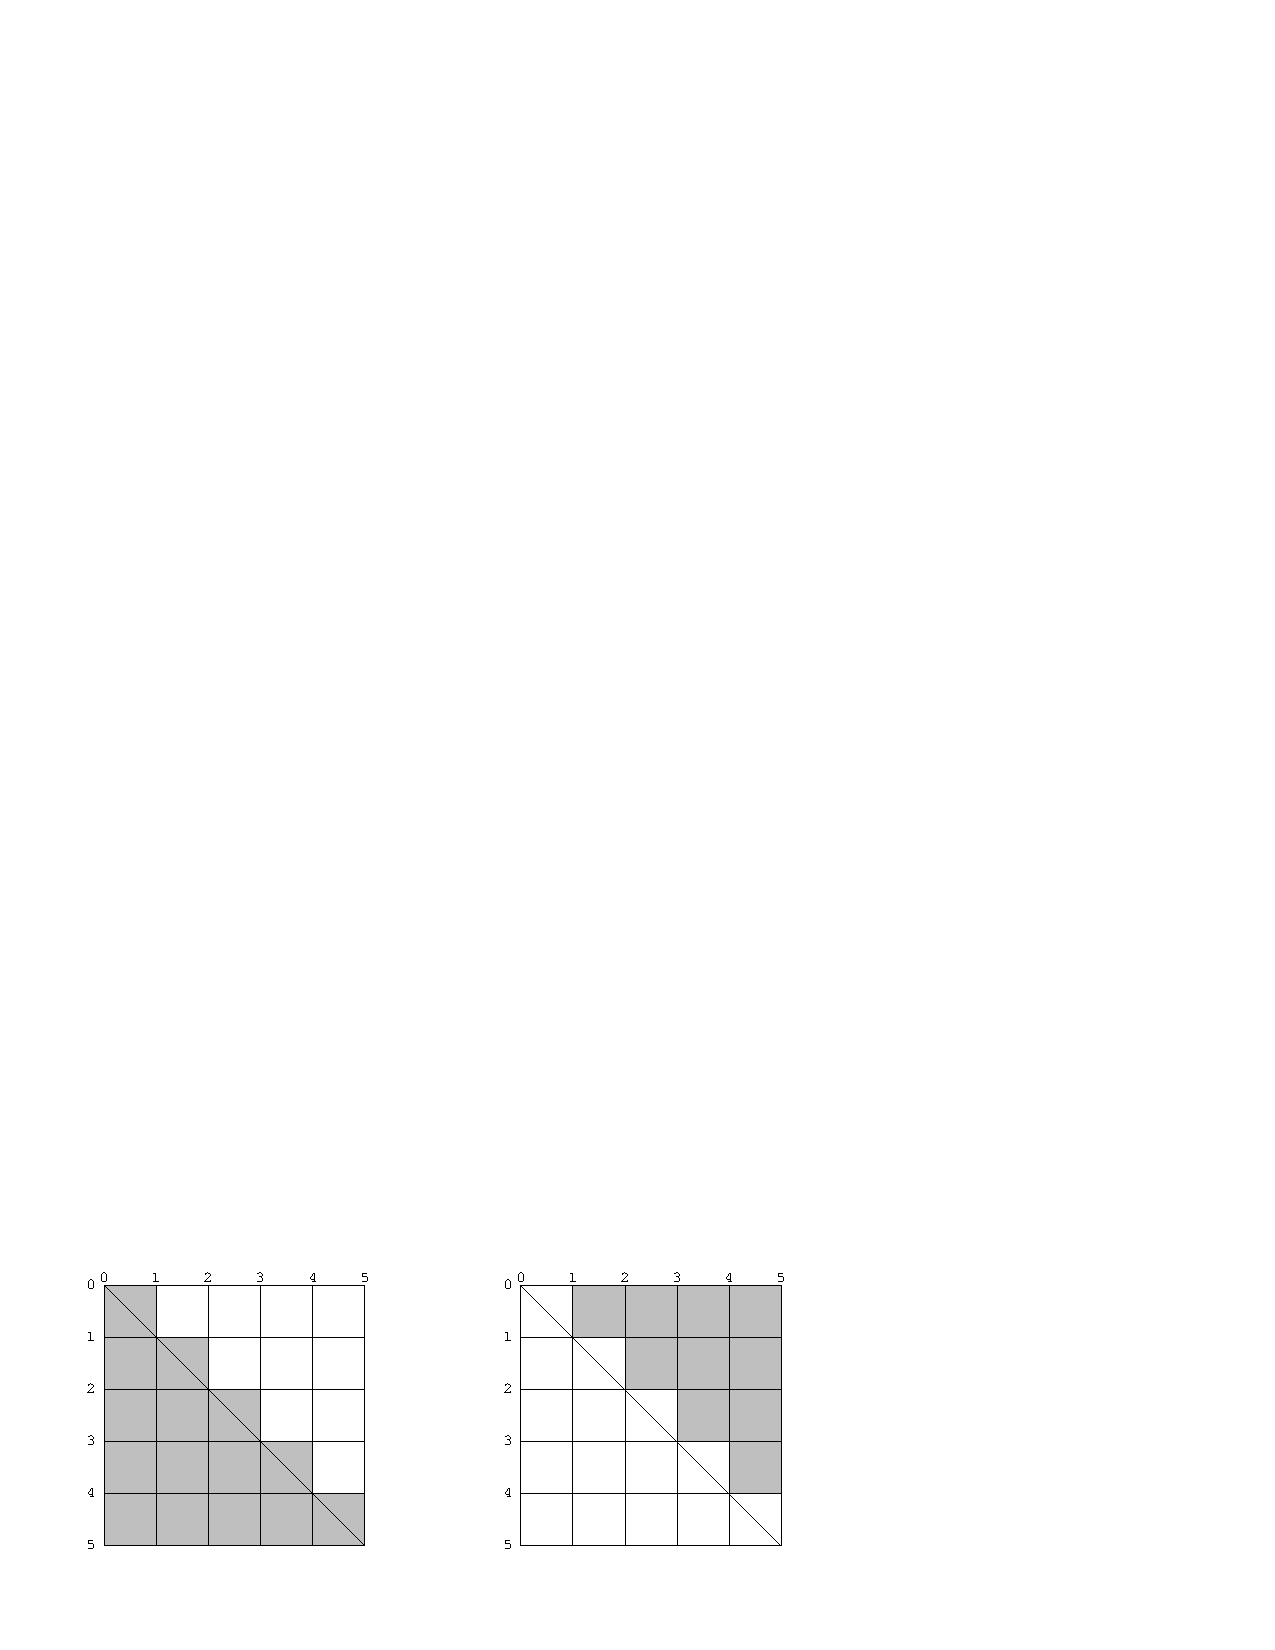
\includegraphics{two-triangles}}
\caption{\label{two-triangles} Pixel assignment with boundary on decision points.}
\end{figure}

The reason for choosing the decision point half a pixel offset from the address
point is to reduce the number of common figures (such as rectilinear lines and
rectangles with integral coordinates) that invoke the boundary condition rule.
This usually leads to more symmetrical results.  For instance, in
Figure~\ref{corner-circle}, we see a circle drawn when the decision point is the
same as the address point.  The four lighter points are indeterminate: it is not
clear whether they are inside or outside the shape.  Since we want to have each
boundary case determined according to which side has the figure on it, and since
we must apply the same rule uniformly for all figures, we have no choice but to
pick only two of the four points, leading to an undesirable lopsided figure.

\begin{figure}
\centerline{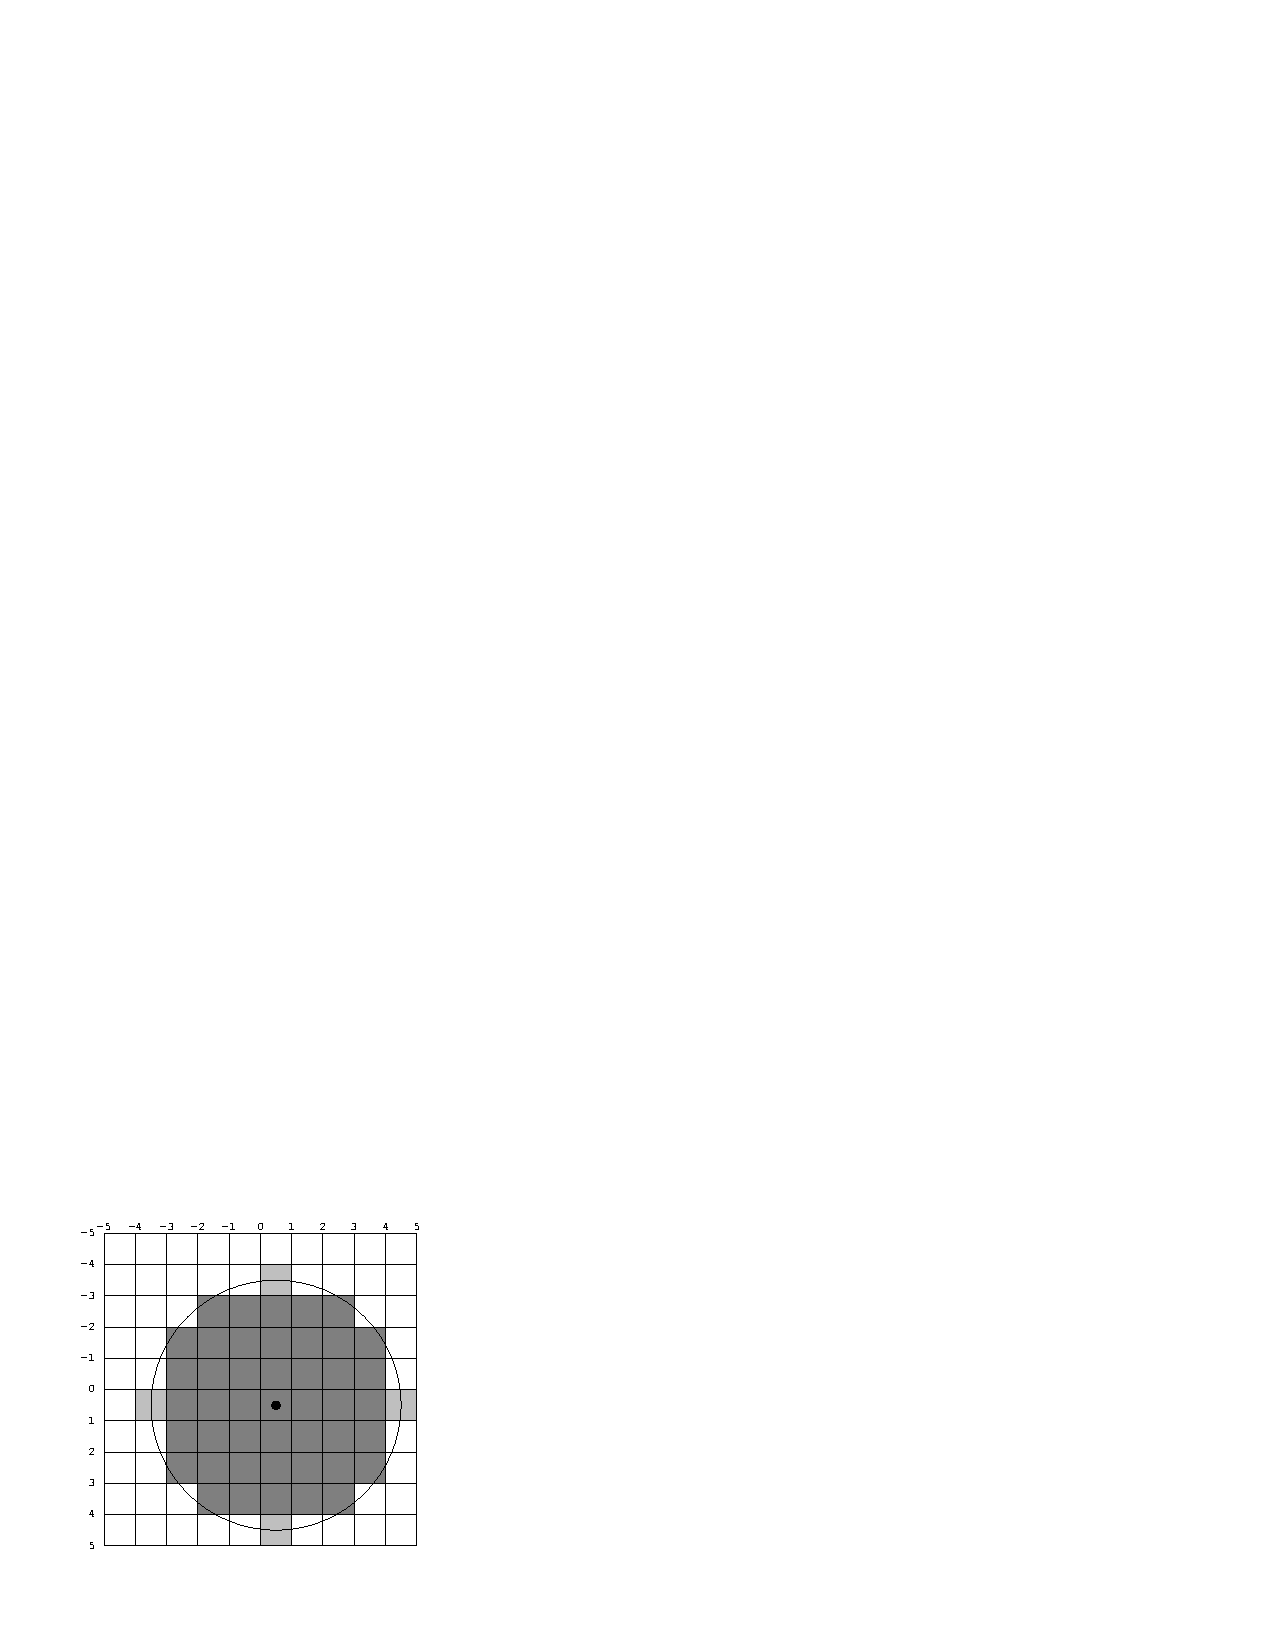
\includegraphics{corner-circle}}
\caption{\label{corner-circle} Choosing any two of the shaded pixels causes asymmetry.}
\end{figure}

If we had instead chosen to take all four boundary points, we would have a nice
symmetrical figure.  However, since this figure is symmetrical about a whole
pixel, it is one pixel wider than it ought to be.  The problem with this can be
seen clearly in Figure~\ref{inscribed-circle} if we attempt to draw a rectangle
and circle overlaid with the following code:

\begin{verbatim}
(defun draw-test (medium radius)
  (draw-circle* medium 0 0 radius :ink +foreground-ink+)
  (draw-rectangle* medium (- radius) (- radius) (+ radius) (+ radius)
                   :ink +flipping-ink+))
\end{verbatim}

\begin{figure}
\centerline{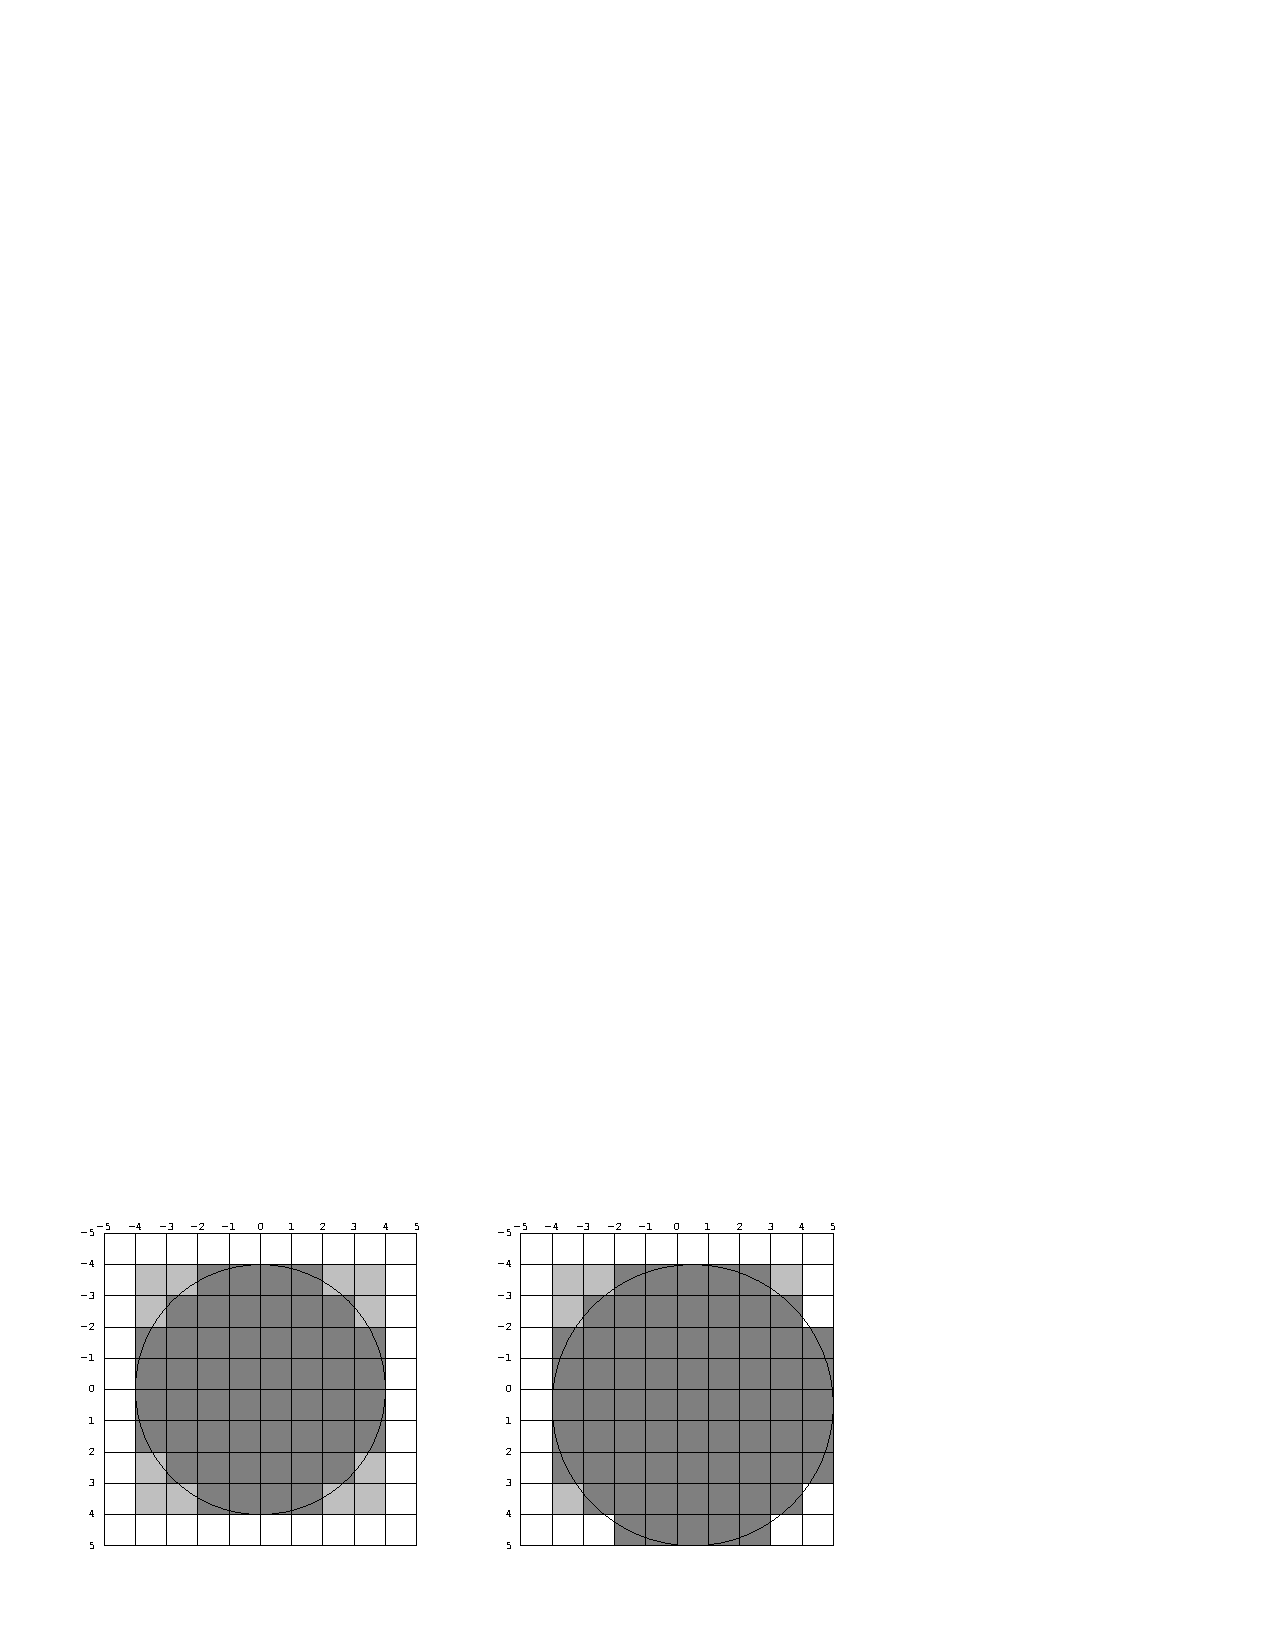
\includegraphics{inscribed-circle}}
\caption{\label{inscribed-circle} Two forms of a circle inscribed in a rectangle.}
\end{figure}

It is for this reason that we choose to have the decision point at the center of
the pixel.  This draws circles that look like the one in
Figure~\ref{correct-circle}.  It is this shape that CLIM implementations should
attempt to draw.

\begin{figure}
\centerline{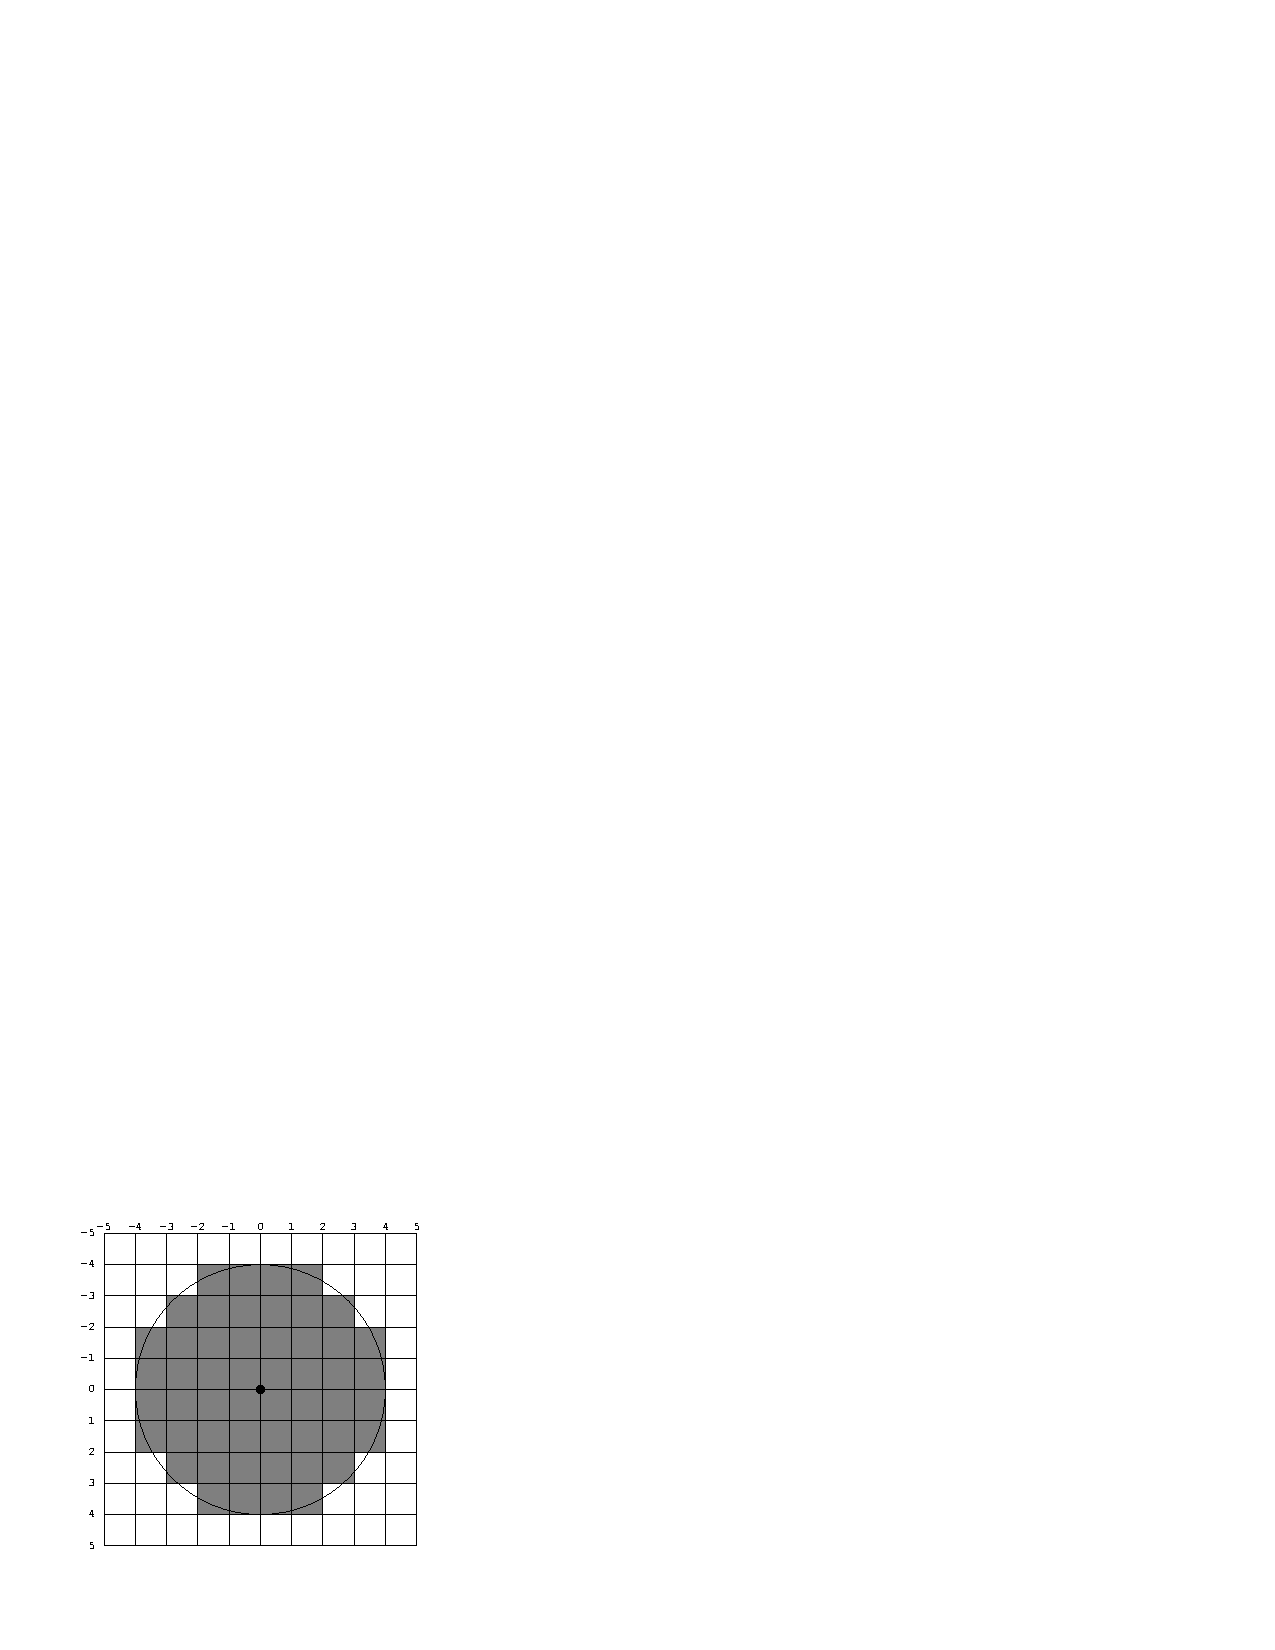
\includegraphics{correct-circle}}
\caption{\label{correct-circle} An aesthetically pleasing circle.}
\end{figure}

A consequence of these rendering conventions is that, when the start or end
coordinate (minus 1/2 the line thickness, if the shape is a path) is not an
integer, then rendering is not symmetric under reflection transformations.  Thus
to correctly and portably draw an outline of thickness 1 around a (rectilinear)
rectangular area with integral coordinates, the outline path must have
half-integral coordinates.  Drawing rectilinear areas whose boundaries are not
on pixel boundaries cannot be guaranteed to be portable.  Another way to say the
same thing is that the ``control points'' for a rectangular area are at the
corners, while the control points for a rectilinear path are in the center of
the path, not at the corners.  Therefore, in order for a path and an area to
abut seamlessly, the coordinates of the path must be offset from the coordinates
of the area by half the path's thickness.

\subsection {Permissible Alternatives During Rendering}

Some platforms may distinguish between lines of the minimum thinness from lines
that are thicker than that.  The two rasterizations depicted in
Figure~\ref{thin-lines} are both perfectly reasonable rasterizations of tilted
lines that are a single device unit wide.  The right-hand line is drawn as a
tilted rectangle, the left as the ``thinnest visible'' line.

\begin{figure}
\centerline{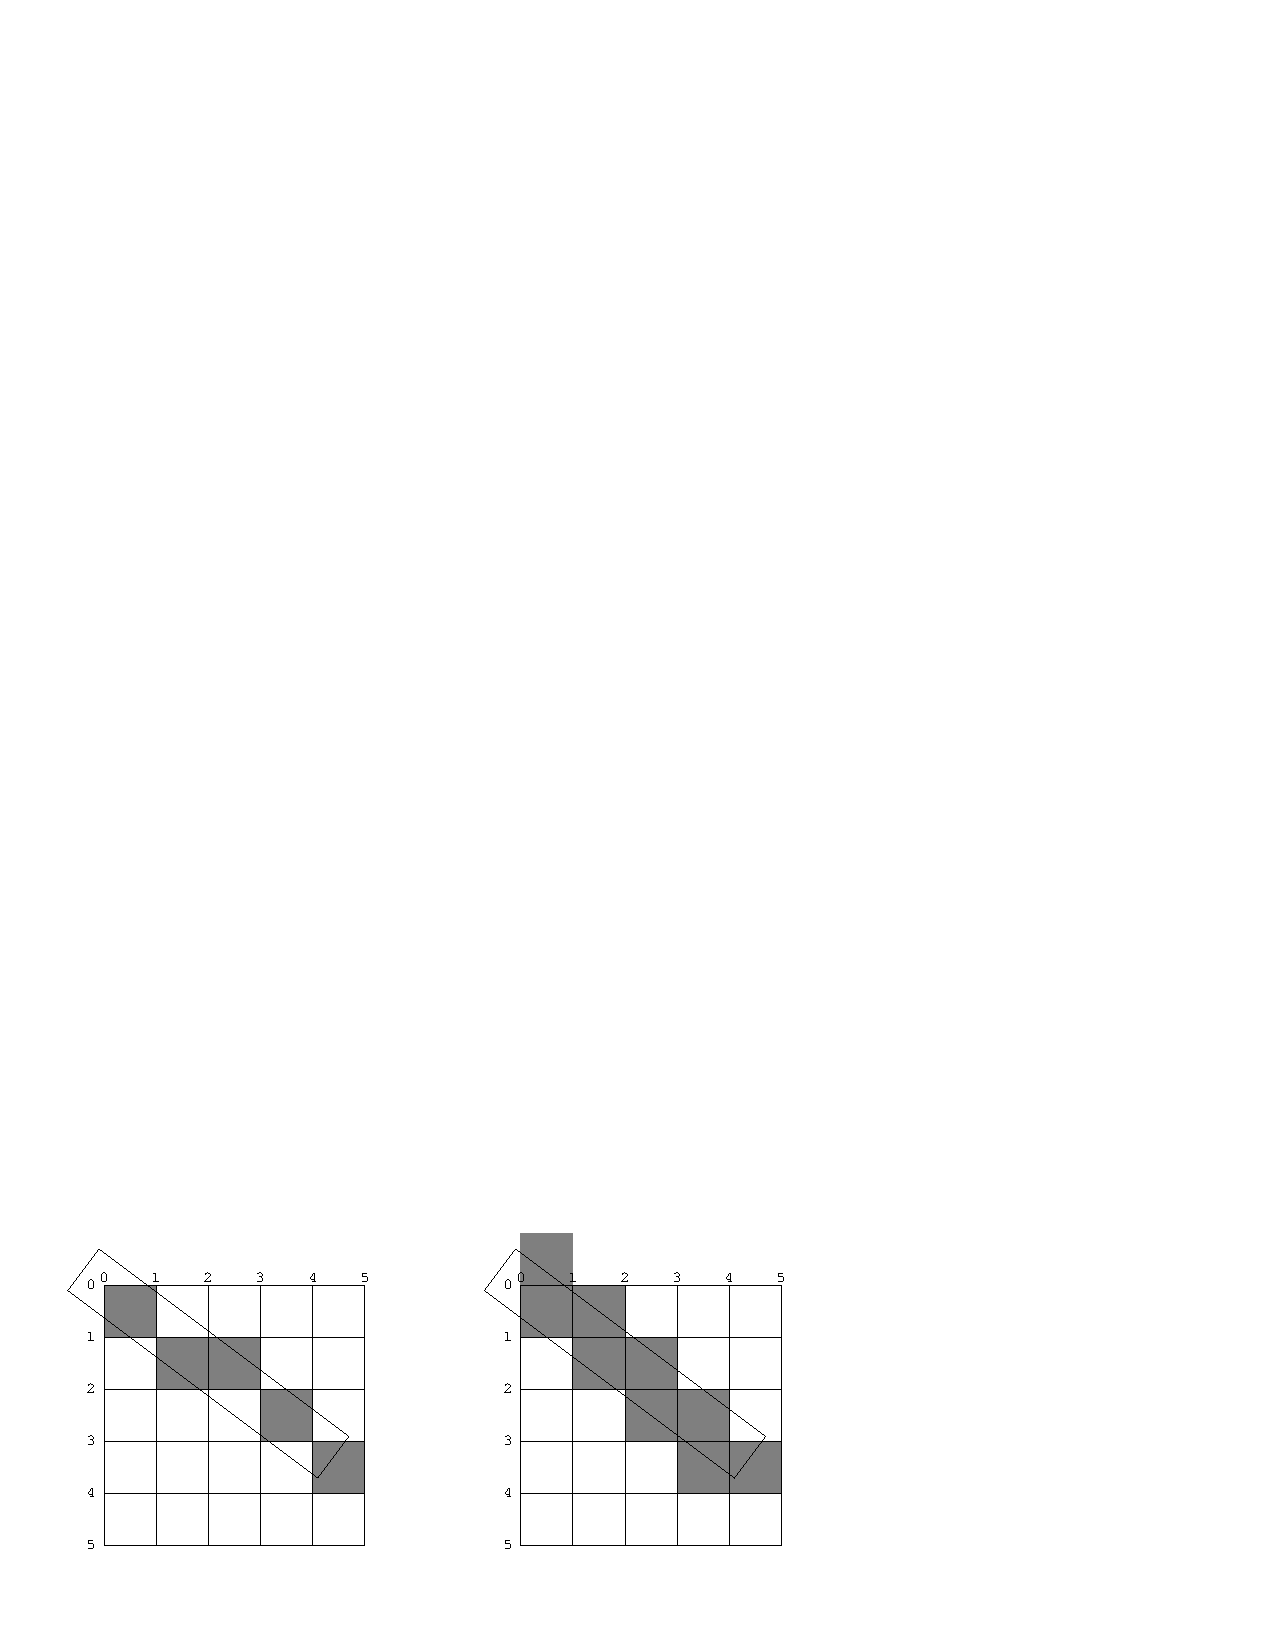
\includegraphics{thin-lines}}
\caption{\label{thin-lines} Two examples of lines of thickness 1.}
\end{figure}

For thick lines, a platform may choose to draw the exact tilted fractional
rectangle, or the coordinates of that rectangle might be rounded so that it is
distorted into another polygonal shape.  The latter case may be prove to be
faster on some platforms.  The two rasterizations depicted in
Figure~\ref{thick-lines} are both reasonable.

\begin{figure}
\centerline{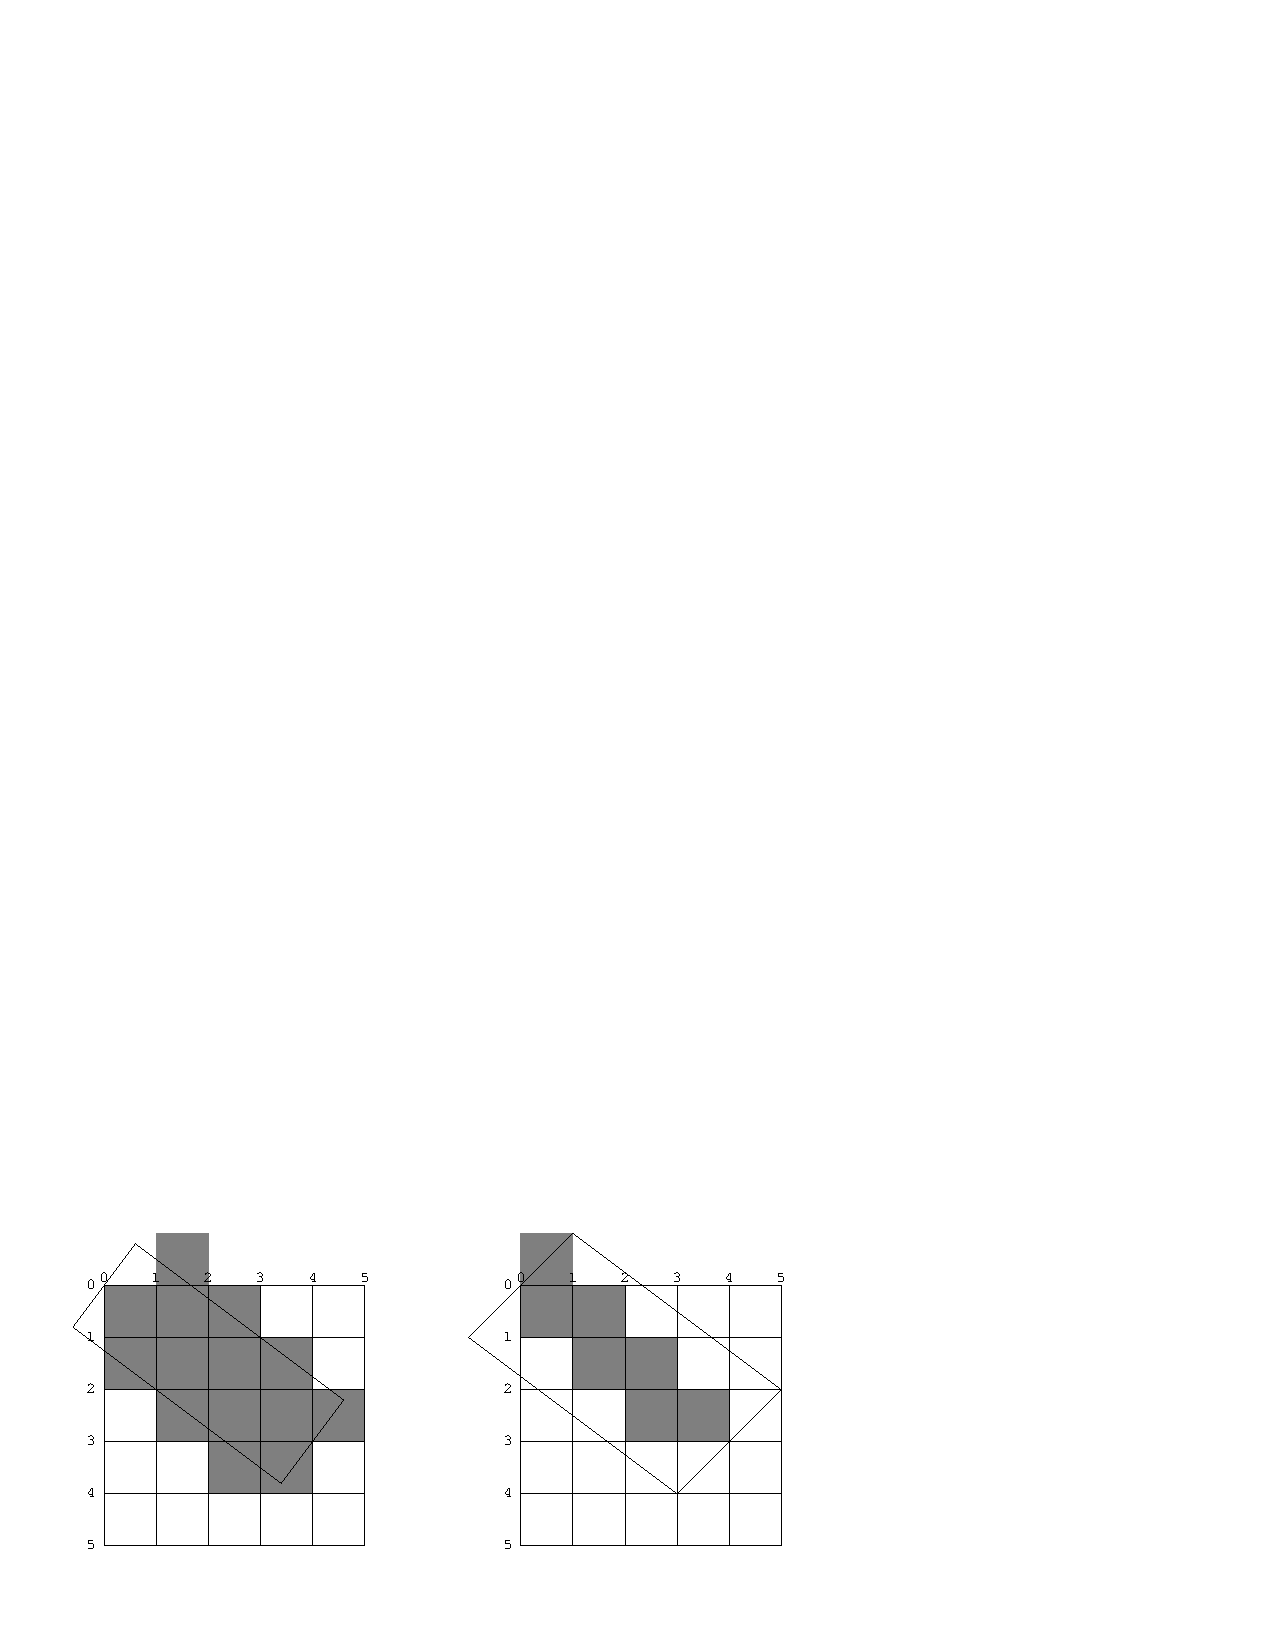
\includegraphics{thick-lines}}
\caption{\label{thick-lines} Two examples of lines of thickness 2.}
\end{figure}

The decision about which side of the shape to take when a boundary line passes
through the decision point is made arbitrarily, although we have chosen to be
compatible with the X11 definition.  This is not necessarily the most convenient
decision.  The main problem with this is illustrated by the case of a horizontal
line (see Figure~\ref{horizontal-lines}).  Our definition chooses to draw the
rectangular slice above the coordinates, since those pixels are the ones whose
centers have the figure immediately above them.  This definition makes it
simpler to draw rectilinear borders around rectilinear areas.

\begin{figure}
\centerline{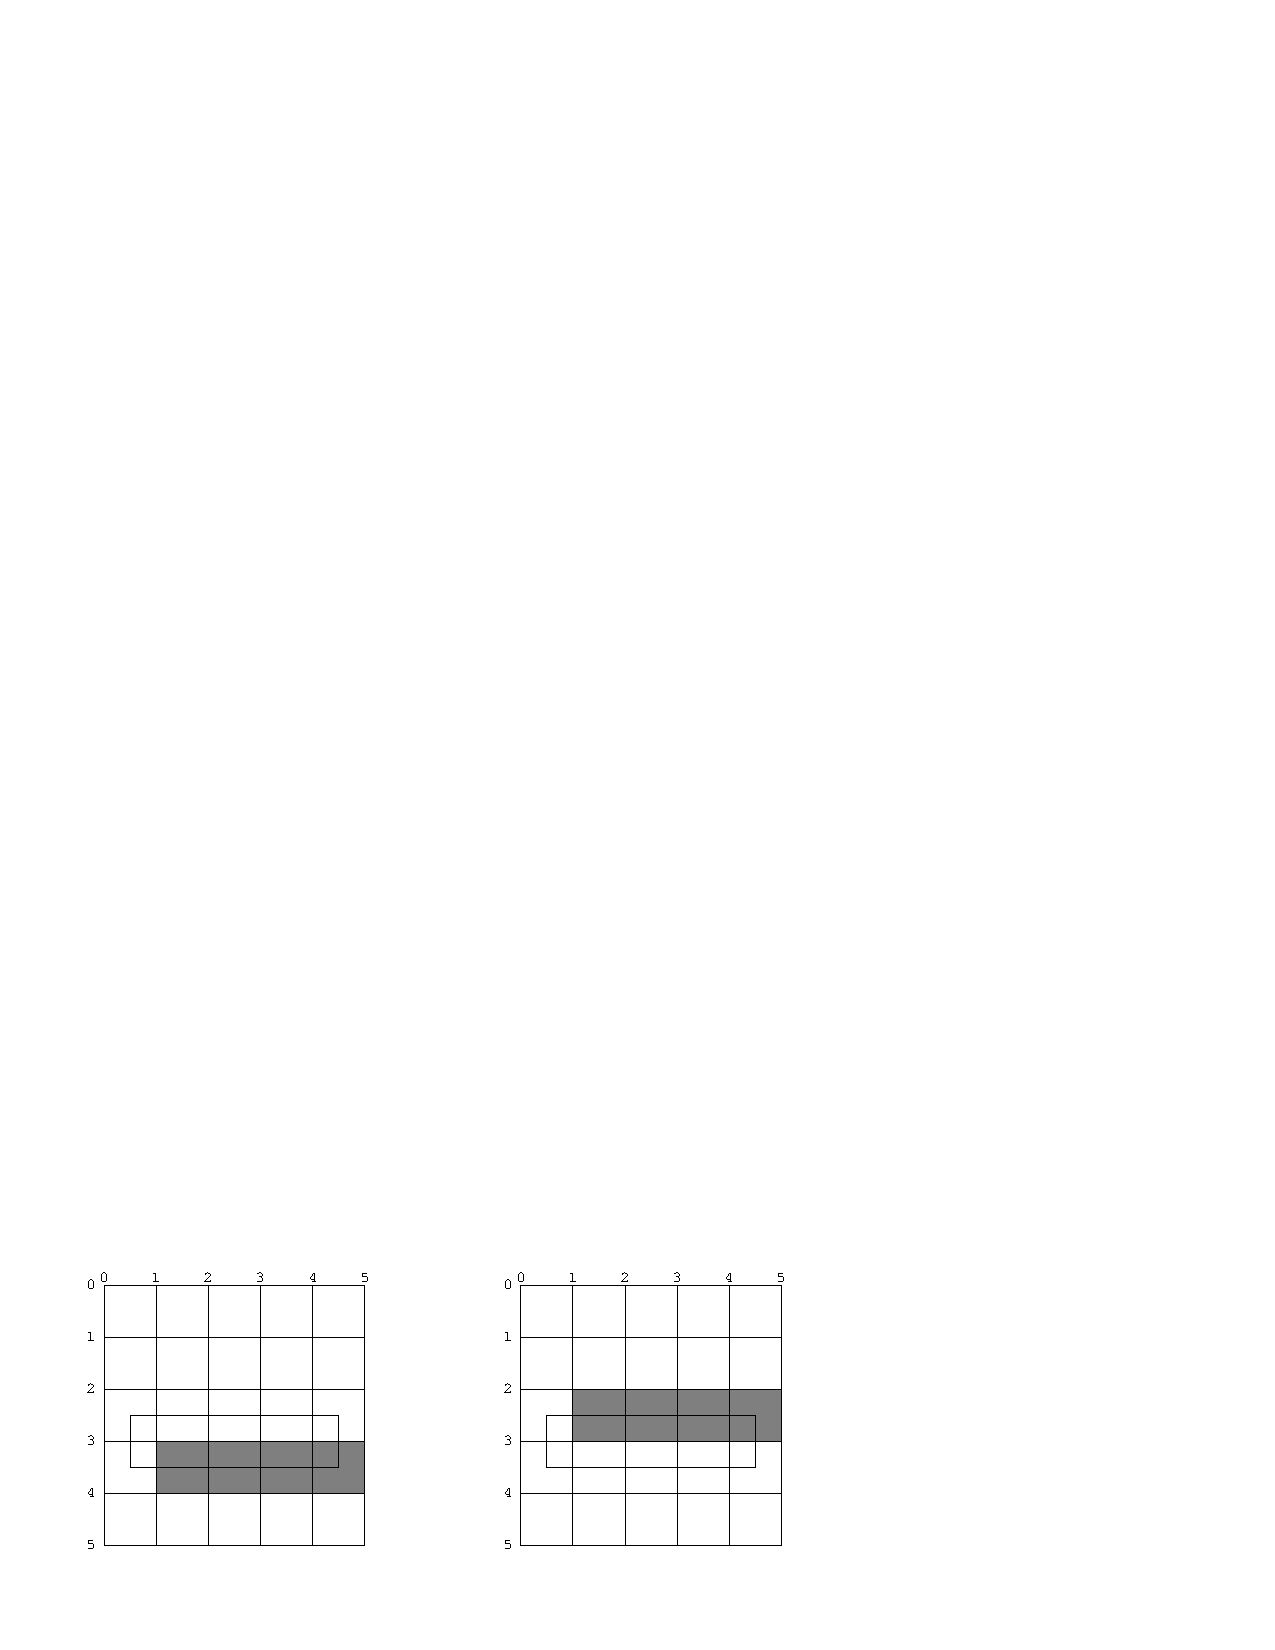
\includegraphics{horizontal-lines}}
\caption{\label{horizontal-lines} Two possible definitions of horizontal lines. 
Left figure is X11 definition.}
\end{figure}


\section {Drawing Functions\label{drawing-functions}}

\def\DrawingOptions{ink clipping-region transformation\ }
\def\PointOptions{line-style line-thickness line-unit}
\def\LineCapOptions{line-style line-thickness line-unit line-dashes line-cap-shape}
\def\LineJointOptions{line-style line-thickness line-unit line-dashes line-joint-shape}
\def\LineJointCapOptions{line-style line-thickness line-unit line-dashes line-joint-shape line-cap-shape}
\def\TextOptions{text-style text-family text-face text-size}

Each drawing function takes keyword arguments allowing any drawing option or
suboption to be supplied separately in the call to the function.  In some
implementations of CLIM, the drawing functions may ignore drawing options that
are irrelevant to that function; in other implementations, an error may be
signalled.  See Chapter~\ref{drawing-options} for a more complete discussion of
the drawing options.  An error will be signalled if any drawing function is
called on a sheet that is mute for output.

While the functions in this section are specified to be called on mediums, they
can also be called on sheets and streams.  CLIM implementations will typically
implement the method on a medium, and write a ``trampoline'' on the various
sheet and stream classes that trampolines to the medium.

{\bf Implementation note:} The drawing functions are all specified as ordinary
functions, not as generic functions.  This is intended to ease the task of
writing compile-time optimizations that avoid keyword argument taking, check for
such things as constant drawing options, and so forth.  If you need to
specialize any of the drawing methods, use \cl{define-graphics-method}.

Each drawing function comes in two forms, a ``structured'' version and a
``spread'' version.  The structured version passes points, whereas the spread
version passes coordinates.  See Section~\ref{spread-vs-point} for more
information on this.

Any drawing functions may create an \term{output record} that corresponds to the
figure being drawn.  See Chapter~\ref{extended-output} for a complete discussion
of output recording.  During output recording, none of these functions capture
any arguments that are points, point sequences, coordinate sequences, or text
strings.  Line styles, text styles, transformations, and clipping regions may be
captured.

Note that the CLIM specification does not specify more complex shapes such as
cubic splines and B\'{e}zier curves.  These are suitable candidates for
extensions to CLIM.


\subsection {Basic Drawing Functions}

\defun {draw-point}  {medium point \key \DrawingOptions \PointOptions}
\Defun {draw-point*} {medium x y   \key \DrawingOptions \PointOptions}

These functions (structured and spread arguments, respectively) draw a single
point on the \term{medium} \arg{medium} at the \term{point} \arg{point} (or the
position $(x,y)$).

The unit and thickness components of the current line style (see
Chapter~\ref{drawing-options}) affect the drawing of the point by controlling
the size on the display device of the ``blob'' that is used to render the point.


\defun {draw-points}  {medium points \key \DrawingOptions \PointOptions}
\Defun {draw-points*} {medium position-seq \key \DrawingOptions \PointOptions}

These functions (structured and spread arguments, respectively) draw a set of
points on the \term{medium} \arg{medium}.  \arg{points} is a sequence of point
objects; \arg{position-seq} is a sequence of coordinate pairs, which are real
numbers.  It is an error if \arg{position-seq} does not contain an even number
of elements.

Ignoring the drawing options, these functions exist as equivalents to
\begin{verbatim}
(map nil #`(lambda (point) (draw-point medium point)) points)
\end{verbatim}
and
\begin{verbatim}
(do ((i 0 (+ i 2)))
    ((= i (length position-seq)))
  (draw-point* medium (elt position-seq i) (elt position-seq (+ i 1))))
\end{verbatim}
for convenience and efficiency.


\defun {draw-line}  {medium point1 point2 \key \DrawingOptions \LineCapOptions}
\Defun {draw-line*} {medium x1 y1  x2 y2  \key \DrawingOptions \LineCapOptions}

These functions (structured and spread arguments, respectively) draw a line
segment on the \term{medium} \arg{medium} from the \term{point} \arg{point1} to
\arg{point2} (or from the position (\arg{x1},\arg{y1}) to (\arg{x2},\arg{y2})).

The current line style (see Chapter~\ref{drawing-options}) affects the drawing
of the line in the obvious way, except that the joint shape has no effect.
Dashed lines start dashing at \arg{point1}.


\defun {draw-lines}  {medium points \key \DrawingOptions \LineCapOptions}
\Defun {draw-lines*} {medium position-seq \key \DrawingOptions \LineCapOptions}

These functions (structured and spread arguments, respectively) draw a set of
disconnected line segments.  \arg{points} is a sequence of point objects;
\arg{position-seq} is a sequence of coordinate pairs.  It is an error if
\arg{position-seq} does not contain an even number of elements.

Ignoring the drawing options, these functions are equivalent to
\begin{verbatim}
(do ((i 0 (+ i 2)))
    ((= i (length points)))
  (draw-line medium (elt points i) (elt points (1+ i))))
\end{verbatim}
and
\begin{verbatim}
(do ((i 0 (+ i 4)))
    ((= i (length position-seq)))
  (draw-line* medium (elt position-seq i)       (elt position-seq (+ i 1))
                     (elt position-seq (+ i 2)) (elt position-seq (+ i 3))))
\end{verbatim}


\defun {draw-polygon}  {medium point-seq \key (filled \cl{t}) (closed \cl{t})
                        \DrawingOptions  \LineJointCapOptions}
\Defun {draw-polygon*} {medium coord-seq \key (filled \cl{t}) (closed \cl{t}) 
                        \DrawingOptions \LineJointCapOptions}

Draws a polygon or polyline on the \term{medium} \arg{medium}.  When
\arg{filled} is \term{false}, this draws a set of connected lines, otherwise it
draws a filled polygon.  If \arg{closed} is \term{true} (the default) and
\arg{filled} is \term{false}, it ensures that a segment is drawn that connects
the ending point of the last segment to the starting point of the first segment.
The current line style (see Chapter~\ref{drawing-options}) affects the drawing
of unfilled polygons in the obvious way.  The cap shape affects only the
``open'' vertices in the case when \arg{closed} is \term{false}.  Dashed lines
start dashing at the starting point of the first segment, and may or may not
continue dashing across vertices, depending on the window system.

\arg{point-seq} is a sequence of point objects; \arg{coord-seq} is a sequence of
coordinate pairs.  It is an error if \arg{coord-seq} does not contain an even
number of elements.

If \arg{filled} is \term{true}, a closed polygon is drawn and filled in.  In
this case, \arg{closed} is assumed to be \term{true} as well.


\Defun {draw-rectangle} {medium point1 point2 \key (filled \cl{t})
                         \DrawingOptions \LineJointOptions}
\Defun {draw-rectangle*} {medium x1 y1 x2 y2 \key (filled \cl{t})
                          \DrawingOptions \LineJointOptions} 

Draws either a filled or unfilled rectangle on the \term{medium} \arg{medium} that
has its sides aligned with the coordinate axes of the native coordinate system.
One corner of the rectangle is at the position (\arg{x1},\arg{y1}) and the
opposite corner is at (\arg{x2},\arg{y2}).  The arguments \arg{x1}, \arg{y1},
\arg{x2}, and \arg{y1} are real numbers that are canonicalized in the same way
as for \cl{make-bounding-rectangle}.  \arg{filled} is as for \cl{draw-polygon*}.

The current line style (see Chapter~\ref{drawing-options}) affects the drawing
of unfilled rectangles in the obvious way, except that the cap shape has no
effect.


\defun {draw-rectangles}  {medium points \key \DrawingOptions \LineJointOptions}
\Defun {draw-rectangles*} {medium position-seq \key \DrawingOptions \LineJointOptions}

These functions (structured and spread arguments, respectively) draw a set of
rectangles.  \arg{points} is a sequence of point objects; \arg{position-seq} is
a sequence of coordinate pairs.  It is an error if \arg{position-seq} does not
contain an even number of elements.

Ignoring the drawing options, these functions are equivalent to
\begin{verbatim}
(do ((i 0 (+ i 2)))
    ((= i (length points)))
  (draw-rectangle medium (elt points i) (elt points (1+ i))))
\end{verbatim}
and
\begin{verbatim}
(do ((i 0 (+ i 4)))
    ((= i (length position-seq)))
  (draw-rectangle* medium (elt position-seq i)       (elt position-seq (+ i 1))
                          (elt position-seq (+ i 2)) (elt position-seq (+ i 3))))
\end{verbatim}


\defun {draw-ellipse}  {medium center-pt radius-1-dx radius-1-dy radius-2-dx radius-2-dy
                        \key (filled \cl{t}) start-angle end-angle
                        \DrawingOptions \LineCapOptions}
\Defun {draw-ellipse*} {medium center-x center-y radius-1-dx radius-1-dy radius-2-dx radius-2-dy
                        \key (filled \cl{t}) start-angle end-angle
                        \DrawingOptions \LineCapOptions}

These functions (structured and spread arguments, respectively) draw an ellipse
(when \arg{filled} is \term{true}, the default) or an elliptical arc (when
\arg{filled} is \term{false}) on the \term{medium} \arg{medium}.  The center of
the ellipse is the \term{point} \arg{center-pt} (or the position
(\arg{center-x},\arg{center-y})).

Two vectors, (\arg{radius-1-dx},\arg{radius-1-dy}) and
(\arg{radius-2-dx},\arg{radius-2-dy}) specify the bounding parallelogram of the
ellipse as explained in Chapter~\ref{regions}.  All of the radii are real
numbers.  If the two vectors are collinear, the ellipse is not well-defined and
the \cl{ellipse-not-well-defined} error will be signalled.  The special case
of an ellipse with its major axes aligned with the coordinate axes can be
obtained by setting both \arg{radius-1-dy} and \arg{radius-2-dx} to 0.

\arg{start-angle} and \arg{end-angle} are real numbers that specify an arc
rather than a complete ellipse.  Angles are measured with respect to the
positive $x$ axis.  The elliptical arc runs positively (counter-clockwise) from
\arg{start-angle} to \arg{end-angle}.  The default for \arg{start-angle} is $0$;
the default for \arg{end-angle} is $2\pi$.

In the case of a ``filled arc'' (that is when \arg{filled} is \term{true} and
\arg{start-angle} or \arg{end-angle} are supplied and are not $0$ and $2\pi$),
the figure drawn is the ``pie slice'' area swept out by a line from the center
of the ellipse to a point on the boundary as the boundary point moves from
\arg{start-angle} to \arg{end-angle}.

When drawing unfilled ellipses, the current line style (see
Chapter~\ref{drawing-options}) affects the drawing in the obvious way, except
that the joint shape has no effect.  Dashed elliptical arcs start ``dashing'' at
\arg{start-angle}.


\defun {draw-circle}  {medium center-pt radius \key (filled \cl{t}) start-angle end-angle
                       \DrawingOptions \LineCapOptions}
\Defun {draw-circle*} {medium center-x center-y radius \key (filled \cl{t}) start-angle end-angle
                       \DrawingOptions \LineCapOptions}

These functions (structured and spread arguments, respectively) draw a circle
(when \arg{filled} is \term{true}, the default) or a circular arc (when
\arg{filled} is \term{false}) on the \term{medium} \arg{medium}.  The center of
the circle is \arg{center-pt} or (\arg{center-x},\arg{center-y}) and the radius
is \arg{radius}.  These are just special cases of \cl{draw-ellipse} and
\cl{draw-ellipse*}.  \arg{filled} is as for \cl{draw-ellipse*}.

\arg{start-angle} and \arg{end-angle} allow the specification of an arc rather
than a complete circle in the same manner as that of the ellipse functions,
above.

The ``filled arc'' behavior is the same as that of an ellipse, above.


\defun {draw-text}  {medium string-or-char point
                     \key text-style (start \cl{0}) end
                          (align-x \cl{:left}) (align-y \cl{:baseline})
                          toward-point transform-glyphs
                     \DrawingOptions \TextOptions}
\Defun {draw-text*} {medium string-or-char x y
                     \key text-style (start \cl{0}) end
                          (align-x \cl{:left}) (align-y \cl{:baseline})
                          toward-x toward-y transform-glyphs
                     \DrawingOptions \TextOptions}

The text specified by \arg{string-or-char} is drawn on the \term{medium}
\arg{medium} starting at the position specified by the \term{point} \arg{point}
(or the position $(x,y)$).  The exact definition of ``starting at'' is dependent
on \arg{align-x} and \arg{align-y}.  \arg{align-x} is one of \cl{:left},
\cl{:center}, or \cl{:right}.  \arg{align-y} is one of \cl{:baseline},
\cl{:top}, \cl{:center}, or \cl{:bottom}.  \arg{align-x} defaults to \cl{:left}
and \arg{align-y} defaults to \cl{:baseline}; with these defaults, the first
glyph is drawn with its left edge and its baseline at \arg{point}.

\arg{text-style} defaults to \cl{nil}, meaning that the text will be drawn using
the current text style of the medium.

\arg{start} and \arg{end} specify the start and end of the string, in the case
where \arg{string-or-char} is a string.  If \arg{start} is supplied, it must be
an integer that is less than the length of the string.  If \arg{end} is
supplied, it must be an integer that is less than the length of the string, but
greater than or equal to \arg{start}.

Normally, glyphs are drawn from left to right no matter what transformation is
in effect.  \arg{toward-x} or \arg{toward-y} (derived from \arg{toward-point} in
the case of \cl{draw-text}) can be used to change the direction from one glyph
to the next one.  For example, if \arg{toward-x} is less than the $x$ position
of \arg{point}, then the glyphs will be drawn from right to left.  If
\arg{toward-y} is greater than the $y$ position of \arg{point}, then the glyphs'
baselines will be positioned one above another.  More precisely, the reference
point in each glyph lies on a line from \arg{point} to \arg{toward-point}, and
the spacing of each glyph is determined by packing rectangles along that line,
where each rectangle is ``char-width'' wide and ``char-height'' high.

If \arg{transform-glyphs} is \term{true}, then each glyph is transformed as an
image before it is drawn.  That is, if a rotation transformation is in effect,
then each glyph will be rotated individually.  If \arg{transform-glyphs} is not
supplied, then the individual glyphs are not subject to the current
transformation.  It is permissible for CLIM implementations to ignore
\arg{transform-glyphs} if it is too expensive to implement.


\subsection {Compound Drawing Functions}

CLIM also provides a few compound drawing functions.  The compound drawing
functions could be composed by a programmer from the basic drawing functions,
but are provided by CLIM because they are commonly used.

\defun {draw-arrow}  {medium point-1 point-2 \key \DrawingOptions \LineCapOptions
                      to-head from-head head-length head-width}
\Defun {draw-arrow*} {medium x1 y1 x2 y2 \key \DrawingOptions \LineCapOptions
                      from-head to-head head-length head-width}

These functions (structured and spread arguments, respectively) draw a line
segment on the \term{medium} \arg{medium} from the \term{point} \arg{point1} to
\arg{point2} (or from the position (\arg{x1},\arg{y1}) to (\arg{x2},\arg{y2})).
If \arg{to-head} is \term{true} (the default), then the ``to'' end of the line
is capped by an arrowhead.  If \arg{from-head} is \term{true} (the default is
\term{false}), then the ``from'' end of the line is capped by an arrowhead.  The
arrowhead has length \arg{head-length} (default 10) and width \arg{head-width}
(default 5).

The current line style (see Chapter~\ref{drawing-options}) affects the drawing
of the line portion of the arrow in the obvious way, except that the joint shape
has no effect.  Dashed arrows start dashing at \arg{point1}.


\defun {draw-oval}  {medium center-pt x-radius y-radius \key (filled \cl{t}) 
                     \DrawingOptions \LineCapOptions}
\Defun {draw-oval*} {medium center-x center-y x-radius y-radius \key (filled \cl{t})
                     \DrawingOptions \LineCapOptions}

These functions (structured and spread arguments, respectively) draw a filled or
unfilled oval (that is, a ``race-track'' shape) on the \term{medium} \arg{medium}.
The oval is centered on \arg{center-pt} (or (\arg{center-x},\arg{center-y})).
If \arg{x-radius} or \arg{y-radius} is $0$, then a circle is drawn with the
specified non-zero radius.  Other, a figure is drawn that results from drawing a
rectangle with dimension {x-radius} by \arg{y-radius}, and the replacing the two
short sides with a semicircular arc of the appropriate size.


\section {Pixmaps}

A \concept{pixmap} can be thought of as an ``off-screen window'', that is, a
medium that can be used for graphical output, but is not visible on any display
device.   Pixmaps are provided to allow a programmer to generate a piece of
output associated with some display device that can then be rapidly drawn on a
real display device.  For example, an electrical CAD system might generate a
pixmap that corresponds to a complex, frequently used part in a VLSI schematic,
and then use \cl{copy-from-pixmap} to draw the part as needed.

The exact representation of a pixmap is explicitly unspecified.  There
is no interaction between the pixmap operations and output recording,
that is, displaying a pixmap on a sheet or medium is a pure drawing
operation that affects only the display, not the output history.  Some
mediums may not support pixmaps; in this case, an error will be
signalled.


\Defgeneric {allocate-pixmap} {medium width height}

Allocates and returns a pixmap object that can be used on any medium that shares
the same characteristics as \arg{medium}.  (The exact definition of ``shared
characteristics'' will vary from host to host.)  \arg{medium} can be a medium, a
sheet, or a stream.

The resulting pixmap will be at least \arg{width} units wide, \arg{height} units
high, and as deep as is necessary to store the information for the medium.  The
exact representation of pixmaps is explicitly unspecified.

The returned value is the pixmap.

\Defgeneric {deallocate-pixmap} {pixmap}

Deallocates the pixmap \arg{pixmap}.


\defgeneric {pixmap-width}  {pixmap}
\defgeneric {pixmap-height} {pixmap}
\Defgeneric {pixmap-depth}  {pixmap}

These functions return, respectively, the width, height, and depth of the pixmap
\arg{pixmap}.  These values may be different from the programmer-specified
values, since some window systems need to allocate pixmaps only of particular
sizes.


\Defun {copy-to-pixmap} {medium medium-x medium-y width height
                         \optional pixmap (pixmap-x \cl{0}) (pixmap-y \cl{0})}

Copies the pixels from the medium \arg{medium} starting at the position specified
by (\arg{medium-x},\arg{medium-y}) into the pixmap \arg{pixmap} at the position
specified by (\arg{pixmap-x},\arg{pixmap-y}).  A rectangle whose width and
height is specified by \arg{width} and \arg{height} is copied.  \arg{medium-x}
and \arg{medium-y} are specified in user coordinates.  (If \arg{medium} is a
medium or a stream, then \arg{medium-x} and \arg{medium-y} are transformed by the
user transformation.)  The copying must be done by \cl{medium-copy-copy}.

If \arg{pixmap} is not supplied, a new pixmap will be allocated.  Otherwise,
\arg{pixmap} must be an object returned by \cl{allocate-pixmap} that has the
appropriate characteristics for \arg{medium}. 

The returned value is the pixmap.

\Defun {copy-from-pixmap} {pixmap pixmap-x pixmap-y width height
                           medium medium-x medium-y}

Copies the pixels from the pixmap \arg{pixmap} starting at the position
specified by (\arg{pixmap-x},\arg{pixmap-y}) into the medium \arg{medium} at the
position (\arg{medium-x},\arg{medium-y}).  A rectangle whose width and height is
specified by \arg{width} and \arg{height} is copied.  \arg{medium-x} and
\arg{medium-y} are specified in user coordinates.  (If \arg{medium} is a medium or
a stream, then \arg{medium-x} and \arg{medium-y} are transformed by the user
transformation.)  The copying must be done by \cl{medium-copy-copy}.

\arg{pixmap} must be an object returned by \cl{allocate-pixmap} that has the
appropriate characteristics for \arg{medium}.

The returned value is the pixmap.

\Defgeneric {copy-area} {medium from-x from-y width height to-x to-y}

Copies the pixels from the medium \arg{medium} starting at the position
specified by (\arg{from-x},\arg{from-y}) to the position (\arg{to-x},\arg{to-y})
on the same medium.  A rectangle whose width and height is specified by
\arg{width} and \arg{height} is copied.  \arg{from-x}, \arg{from-y}, \arg{to-x},
and \arg{to-y} are specified in user coordinates.  (If \arg{medium} is a medium
or a stream, then the $x$ and $y$ values are transformed by the user
transformation.)  The copying must be done by \cl{medium-copy-copy}.


\Defgeneric {medium-copy-area} {from-drawable from-x from-y width height
                                to-drawable to-x to-y}

Copies the pixels from the source drawable \arg{from-drawable} at the position
(\arg{from-x},\arg{from-y}) to the destination drawable \arg{to-drawable} at the
position (\arg{to-x},\arg{to-y}).  A rectangle whose width and height is
specified by \arg{width} and \arg{height} is copied.  \arg{from-x},
\arg{from-y}, \arg{to-x}, and \arg{to-y} are specified in user coordinates.
The $x$ and $y$ are transformed by the user transformation.

This is intended to specialize on both the \arg{from-drawable} and
\arg{to-drawable} arguments.  \arg{from-drawable} and \arg{to-drawable} may be
either mediums or pixmaps.


\Defmacro {with-output-to-pixmap} {(medium-var medium \key width height) \body body}

Binds \arg{medium-var} to a ``pixmap medium'', that is, a medium that does
output to a pixmap with the characteristics appropriate to the medium
\arg{medium}, and then evaluates \arg{body} in that context.  All the output done
to the medium designated by \arg{medium-var} inside of \arg{body} is drawn on
the pixmap stream.  The pixmap medium must support the medium output protocol,
including all of the graphics function.  CLIM implementations are permitted, but
not required, to have pixmap mediums support the stream output protocol
(\cl{write-char} and \cl{write-string}).

\arg{width} and \arg{height} are integers that give the width and height of the
pixmap.  If they are unsupplied, the result pixmap will be large enough to
contain all of the output done by \arg{body}.

\arg{medium-var} must be a symbol; it is not evaluated.

The returned value is a pixmap that can be drawn onto \arg{medium} using
\cl{copy-from-pixmap}.


\section {Graphics Protocols\label{graphics-protocols}}

Every medium must implement methods for the various graphical drawing generic
functions.  Furthermore, every sheet that supports the standard output protocol
must implement these methods as well; often, the sheet methods will trampoline
to the methods on the sheet's medium.  All of these generic functions take the
same arguments as the non-generic spread function equivalents, except the
arguments that are keyword arguments in the non-generic functions are positional
arguments in the generic functions.

Every medium must implement methods for the various graphical drawing generic
functions.  All of these generic functions take as (specialized) arguments the
medium, followed by the drawing function-specific arguments, followed by the
ink, line style (or text style), and clipping region.

The drawing function-specific arguments will either be $x$ and $y$ positions,
or a sequence of $x$ and $y$ positions.  These positions will be in medium
coordinates, and must be transformed by applying the medium's device
transformation in order to produce device coordinates.  Note that the user
transformation will have already been applied to the positions when the
medium-specific drawing function is called.  However, the medium-specific
drawing function will still need to apply the device transformation to the
positions in order to draw the graphics in the appopriate place on the host
window.

The ink, line style, text style, and clipping regions arguments are not part of
the medium-specific drawing functions.  They must be extracted from the medium
object.  Each medium-specific method will decode the ink, line (or text) style,
and clipping region in a port-specific way and communicate it to the underlying
port.


\subsection {General Behavior of Drawing Functions}

Using \cl{draw-line*} as an example, calling any of the drawing functions
specified above results in the following series of function calls on a
non-output recording sheet:

\begin{itemize} 
\item A program calls \cl{draw-line*} on either a sheet or a medium, \arg{x1},
\arg{y1}, \arg{x2}, and \arg{y2}, and perhaps some drawing options.

\item \cl{draw-line*} merges the supplied drawing options into the medium, and
then calls \cl{medium-draw-line*} on the sheet or medium.  (Note that a compiler
macro could detect the case where there are no drawing options or constant
drawing options, and do this at compile time.)

\item If \cl{draw-line*} was called on a sheet, the \cl{medium-draw-line*} on
the sheet trampolines to the medium's \cl{medium-draw-line*} method.

\item An \cl{:around} method for \cl{medium-draw-line*} performs the necessary
user transformations by applying the medium transformation to \arg{x1},
\arg{y1}, \arg{x2}, and \arg{y2}, and to the clipping region, and then calls the
medium-specific method.

\item The ``real'' \cl{medium-draw-line*} transforms the start and end
coordinates of the line by the sheet's device transformation, decodes the ink
and line style into port-specific objects, and finally invokes a port-specific
function (such as \cl{xlib:draw-line}) to do the actual drawing.
\end{itemize}


\subsection {Medium-specific Drawing Functions}

All mediums and all sheets that support the standard output protocol must
implement methods for the following generic functions.

The method for each of these drawing functions on the most specific,
implementation-dependent medium class will transform the coordinates by the
device transformation of the medium's sheet, extract the medium's port-specific
``drawable'', and then invoke a port-specific drawing function (such as
\cl{xlib:draw-line}) to do the actual drawing.

An \cl{:around} on \cl{basic-medium} for each of the drawing functions will have
already transformed the user coordinates to medium coordinates before the most
specific, implementation-dependent method is called.

{\bf Implementation note:} CLIM implementations should provide ``trampoline''
methods on sheets that support the standard output protocol that simply call the
same generic function on the medium.  Sheets that support output recording will
require extra mechanism before delegating to the medium in order to implement
such functionality as creating output records and handling scrolling.

\Defgeneric {medium-draw-point*} {medium x y}

Draws a point on the \term{medium} \arg{medium}.  

\Defgeneric {medium-draw-points*} {medium coord-seq}

Draws a set of points on the \term{medium} \arg{medium}.  \arg{coord-seq} is a
sequence of coordinate pairs, which are real numbers.  It is an error if
\arg{coord-seq} does not contain an even number of elements.

\Defgeneric {medium-draw-line*} {medium x1 y1 x2 y2}

Draws a line on the \term{medium} \arg{medium}.  The line is drawn from
$(x1,y1)$ to $(x2,y2)$.

\Defgeneric {medium-draw-lines*} {stream position-seq} 

Draws a set of disconnected lines on the \term{medium} \arg{medium}.
\arg{coord-seq} is a sequence of coordinate pairs, which are real numbers.  Each
successive pair of coordinate pairs is taken as the start and end position of
each line.  It is an error if \arg{coord-seq} does not contain an even number of
elements.

\Defgeneric {medium-draw-polygon*} {medium coord-seq closed}

Draws a polygon or polyline on the \term{medium} \arg{medium}.  \arg{coord-seq}
is a sequence of coordinate pairs, which are real numbers.  It is an error if
\arg{coord-seq} does not contain an even number of elements.  Each successive
coordinate pair is taken as the position of one vertex of the polygon.

\Defgeneric {medium-draw-rectangle*} {medium x1 y1 x2 y2}

Draws a rectangle on the \term{medium} \arg{medium}.  The corners of the
rectangle are at $(x1,y1)$ and $(x2,y2)$.

\Defgeneric {medium-draw-rectangles*} {medium coord-seq}

Draws a set of rectangles on the \term{medium} \arg{medium}.  \arg{coord-seq} is
a sequence of coordinate pairs, which are real numbers.  It is an error if
\arg{coord-seq} does not contain an even number of elements.  Each successive
pair of coordinate pairs is taken as the upper-left and lower-right corner of
the rectangle.

\Defgeneric {medium-draw-ellipse*} {medium center-x center-y 
                                    radius-1-dx radius-1-dy radius-2-dx radius-2-dy  
                                    start-angle end-angle}


Draws an ellipse or elliptical arc on the \term{medium} \arg{medium}.  The
center of the ellipse is at $(x,y)$, and the radii are specified by the two
vectors (\arg{radius-1-dx},\arg{radius-1-dy}) and
(\arg{radius-2-dx},\arg{radius-2-dy}).

\arg{start-angle} and \arg{end-angle} are real numbers that specify an arc
rather than a complete ellipse.  Note that the medium and device transformations
must be applied to the angles as well.

\Defgeneric {medium-draw-text*} {medium text x y
                                 (start \cl{0}) end
                                 (align-x \cl{:left}) (align-y \cl{:baseline})
                                 toward-x toward-y transform-glyphs}

Draws a character or a string on the \term{medium} \arg{medium}.  The text is
drawn starting at $(x,y)$, and towards (\arg{toward-x},\arg{toward-y}).  In Some
implementations of CLIM, \cl{medium-draw-text*} may call either
\cl{medium-draw-string*} or \cl{medium-draw-character*} in order to draw the
text.

\subsection {Other Medium-specific Output Functions}

\Defgeneric {medium-finish-output} {medium}

Ensures that all the output sent to \arg{medium} has reached its destination,
and only then return \term{false}.  This is used by \cl{finish-output}.

\Defgeneric {medium-force-output} {medium}

Like \cl{medium-finish-output}, except that it may return \term{false} without
waiting for the output to complete.  This is used by \cl{force-output}.

\Defgeneric {medium-clear-area} {medium left top right bottom}

Clears an area on the {medium} \arg{medium} by filling the rectangle whose edges
are at \arg{left}, \arg{top}, \arg{right}, and \arg{bottom} with the medium's
background ink.  \arg{left}, \arg{top}, \arg{right}, and \arg{bottom} are in
thed medium's coordinate system.

The default method on \cl{basic-medium} simply uses \cl{draw-rectangle*} to
clear the area.  Some host window systems has special functions that are faster
than \cl{draw-rectangle*}.

\Defgeneric {medium-beep} {medium}

Causes an audible sound to be played on the medium.  The default method
does nothing.

